% Author: Bernard Lampe

% Use the IEEE classes
\documentclass[journal]{IEEEtran}

% Packages
\usepackage[cmex10]{amsmath}
\usepackage{url}
\usepackage{cite}
\usepackage{graphicx}
\usepackage{subfig}
\usepackage{float}

% Correct bad hyphenation here
\hyphenation{op-tical net-works semi-conduc-tor}
\DeclareMathOperator*{\argmax}{arg\,max}
\DeclareMathOperator*{\argmin}{arg\,min}

% Start document
\begin{document}

% Paper title
\title{Linear Discriminant Functions for Classification}

% Author
\author{Bernard~Lampe,~\IEEEmembership{Member,~IEEE}}

% The paper headers
\markboth{Linear Discriminant Functions for Classifications}
{Shell \MakeLowercase{\Lampe}: Linear Discriminant Functions for Classification}

% Make the title area
\maketitle

\begin{abstract}
In this study we demonstrate two linear classification techniques using Fisher's Linear Discriminant Analysis (FLDA) and Support Vector Machine (SVM). We begin with classifier design using supervised learning and the two class problem. Then we extend to the multiple class problem by applying the two class classifier employing the heuristics of one-to-one and one-to-all. By constructing classifiers based on the two class problem we will encounter regions of ambiguous class assignment during testing. To mitigate these ambiguous classifications we demonstrate several separate heuristics. Additionally, we design a multiple class classifier using the natural generalization of FLDA and the Orthogonal Subspace Projection (OSP). Finally, we compute classification rates of each designed classifier and make anecdotal observations of the classifier effectiveness in our problem domain. All data used for the experiments and training were generated via a parametrized Bernoulli distribution (biased coins).
\end{abstract}

% Keywords
\begin{IEEEkeywords}
Two-class Classification, Multi-class Classification, Fisher Linear Discriminant Analysis, Support Vector Machine, Maximum Likelihood Classification, FLDA, SVM, MLE
\end{IEEEkeywords}

% Introduction with drop letter and first word capitalized.
\section{Introduction}

\IEEEPARstart{T}{he} optimal decision rule for classifying new test samples, denoted \(\vec{x}\), into one of \(K\) classes, denoted \(C_k\), is based on choosing the class which maximizes the joint probability between sample features and the class such that \(p(\vec{x}, C_j) > p(\vec{x}, C_k)\) for all \(j \ne k\). These joint probabilities are rarely known aprior when designing classifiers for real world applications. Therefore, they are often estimated using training data and one of several parametric or non-parametric density estimation techniques which are thoroughly covered in the literature \cite[p.~33-73]{bishop1}\cite[p.~20-213]{duda}. Density estimation of the class priors, \(p(C_k)\), the class conditionals, \(p(\vec{x}|C_k)\) or the posterior probabilities, \(p(C_k|\vec{x})\), is sensitive to the quality and number of training samples as well as the estimation technique used. The aforementioned approach separates classifier design into two steps, probability density inference followed by a decision rule. A simpler approach which combines both inference and the decision rule is to use the training data to find a discriminant function \(y(\vec{x})\) which will map a new test sample \(\vec{x}\) directly to a class label \(C_k\) \cite[p.~44]{bishop2}.

\par A discriminant function is a parametrized functional form which specifies the decision boundary between classes. The parameters are directly estimated from the training data and are chosen to optimize objective measures which correlate with good class separation in practice. The simplest and most widely used discriminant function form is the linear function as in equation \ref{eq:lineq}. Where \(\vec{w}\) and \(w_0\) are estimated from the training data. The vector \(\vec{w}\) specifies the hyperplane which separates classes and the parameter \(w_0\) specifies the offset of the hyperplane from the origin and is referred to as a threshold or a classifier bias. This linear model is the functional form from which linear classifiers can be designed using FLDA and SVM.

\begin{equation}
\label{eq:lineq}
y(\vec{x}) = \vec{w}^T\vec{x} + w_0
\end{equation}

% Describe Experiments
\section{Training Data and Test Sample Generation}
\par In this study the training data was simulated by flipping a hypothetical coin \(d=100\) times. The training observations were labeled with the target value \(t = k\) which indexes the class \(C_k\). We consider the five class problem and the data was generated by flipping five different, biased coins. The biases are in the set \(\Theta = \{0.1, 0.2, 0.3, 0.4, 0.5\}\). The data pool consists of 3000 samples each of 100 flips such that \(\Delta_k = \{\vec{x}_k^j\}_{j=1}^{200k}\) and \(\Delta = \cup_{k=1}^5{\Delta_k}\). Therefore, 200 samples will be from coin \(k=1\) and \(\theta_{k=1} = 0.1\), 400 samples will be from coin \(k=2\) and \(\theta_{k=2} = 0.2\), etc. The n-th training sample of \(\Delta\) is a tuple of the sample vector and target value \((\vec{x}^n, t^n)\).

\section{Two Class Problem using FLDA}
\par FLDA for the two class and multi-class problem is covered in several well known literature sources so we will only treat the subject briefly here \cite[p.~124-128]{alpaydin}\cite[p.~105-112]{bishop1}\cite[p.~186-192]{bishop2}\cite[p.~117-124]{duda}.

\par The classification problem addressed in this study, with \(d=100\), suffers from what is called the curse of dimensionality. In short, this curse is a practical observation that in order to build an effective classifier for a linearly increasing number of dimensions, an exponential amount of training samples will be required. FLDA addresses this problem by finding a lower dimensional orthogonal subspace upon which the training and test data is projected while preserving good discrimination. Good discrimination is defined by finding the subspace \(\vec{w}\) such that the projected means of each class will be maximally separated while the individual class variances will be minimized. The objective criteria for the two class problem is reproduced here in equations \ref{eq:flda_2}, \ref{eq:flda_mean} and \ref{eq:flda_scatter}. Where \(N_k\) is the number of samples in class \(k\), \(m_k\) is the projected class mean and \(s_k\) is the unnormalized projected class variance known as the scatter. The closed formed solution for finding the optimal \(\vec{w}\) is given in the sources cited earlier. It is worth noting that FLDA is not optimal for all configurations of class data, and is most effective when the covariance of the classes is isotropic \cite[p.~108]{bishop1}.

\begin{equation}
\label{eq:flda_2}
J(\vec{w}) = \frac{(m_2-m_1)^2}{s_1^2+s_2^2}
\end{equation}

\begin{equation}
\label{eq:flda_mean}
m_k = \vec{w}^T\vec{m}_k \text{      and       } \vec{m}_k = \frac{1}{N_k}\sum_{n \in C_k}{\vec{x}^n}
\end{equation}

\begin{equation}
\label{eq:flda_scatter}
s_k^2 = \sum_{n \in C_k}{(y(\vec{x}^n) - m_k)^2}
\end{equation}

\par Therefore, strictly speaking, FLDA is not a classifier, but a dimensionality reduction algorithm. However, it can be easily used to build a classifier by projecting the data onto \(\vec{w}\) and then finding a suitable threshold in the lower dimensional space. In our experiments we used two different methods to perform classification. Firstly, we choose the threshold to be the mid-point of the projected class means. Upon classifying a new data sample, we projected the test sample onto \(\vec{w}\) and choose the class where the Euclidean distance to the mean was minimized as in equation \ref{eq:mids}. The first metric was adequate in many cases and even optimal when the classes demonstrated equal variances. This first metric is mathematically equivalent to using the linear discriminant function in the projected space that minimizes the Least Squared Error (LSE) rate of misclassification. \cite[p.~189-190]{bishop2}. In addition we used a metric which took into account the first and second moments of the projected training data by fitting Gaussian distributions and finding the intersection of the functions. When classifying a new data sample using the second method, we choose class \(C_k\) as the maximum of the Gaussian function of the projected data as in equation \ref{eq:gausss}. This is equivalent to using a MLE classifier with the class conditionals, \(p(\vec{w}^T\vec{x}^n|C_k) \forall n \in C_k\) modeled by a single Gaussian distribution.

\begin{equation}
\label{eq:mids}
f(\vec{x}) = \argmin_{C_k}\| \vec{w}^T\vec{x} - m_k \|_2
\end{equation}

\begin{equation}
\label{eq:gausss}
f(\vec{x}) = \argmax_{C_k}\frac{1}{\sigma_k\sqrt{2\pi}}\exp{-\frac{(\vec{w}^T\vec{x} - m_k)^2}{2\sigma_k^2}}, \sigma_k^2 = \frac{1}{N_k}s_k^2
\end{equation}

In our experiments for the two class problem, \(\vec{w}\) will be a straight line in a \(100\) dimensional space upon which we will project the data to a one dimensional subspace and perform classification there.

\subsection{One-to-One and One-to-All Classification Using FLDA}
\par To extend the two class FLDA classifier we constructed in the prior section to multiple classes we can decompose the \(K\)-classes of the training data into pairs of classes. Two natural pairings are classifying all pairs in a one-to-one strategy or by classifying pairs in a one-to-all strategy.
\par To design a classifier using the one-to-one strategy on a \(K\) class problem, we must solve \(K \choose 2\)\( = K(K-1)/2\ \text{  where  } K = 5\) two class problems resulting in \(10\) classifiers to compute from the training data. Each classifier will have a different projection vector \(\vec{w}_{jk} \text{ for all classes } j \ne k\), projected means \(m_k\), projected variances \(\sigma_k^2\) and thresholds. When classifying a novel sample \(\vec{x}\) using this strategy we will obtain \(10\) class labels for this sample. To resolve the ambiguity, we use a voting strategy and choose the class which received the most votes. While this was highly effective in practice, it does result in some classifications which are assigned to more than one class (i.e. a tie vote). We developed three heuristics to resolve ambiguities and are described later in this paper.
\par To design a multi-class classifier using the one-to-all strategy, we must solve the two class problem \(K\) times. When classifying a new sample, we  must decide if the sample is in class \(C_k\) or not in class \(C_k\) for all \(K\) classes. This is computationally simpler than the one-to-one strategy as the number of classifiers to compute is linear with the number of classes. When classifying a novel sample we compute \(K = 5\) class labels and then choose a class based on those \(5\) labels. This can result in ambiguities where either all \(5\) classifiers result in a "not class \(C_k\)" decision or the sample is assigned to more than one class.
\par In an attempt to resolve ambiguous classifications when using the one-to-one or one-to-all strategy, we developed several heuristics to help improve the classification rate. The first was to simply ignore the samples which have ambiguous labels. The second was to label the test sample with the class that had the highest prior probability and the last was to choose the class label whereby the sample had the smallest \(L_2\) norm to the projected class means.

\subsection{Generalized Multi-Class FLDA and OSP}
\par For the multi-class classifier design problem FLDA has a generalization to an arbitrary number of classes which can be used to compute \(K-1\) feature vectors which are of \(d\) dimension. This results in a considerable dimensionality reduction of our problem from \(d=100\) to \(d=4\). The derivation of the multi-class FLDA is quite involved and beyond the scope of this paper and can be found in several well known sources \cite[p.~110-112]{bishop2}\cite[p~.121-124]{duda}. The result of the analysis is a \(d\) by \(K-1\) projection matrix where by the lower dimension samples are found via \(y(\vec{x}) = W^T\vec{x}\).
\par To compute the projection matrix \(W\) we have to maximize the Fisher's ratio for multiple classes by finding the eigenvectors of the inverted within class scatter matrix. This matrix may be ill-conditioned for inversion if there are few linearly independent samples when compared to dimensionality of the original data \(d\). To overcome this limitation, Harsanyi and Chang \cite[p.~47-48]{chang2} developed an algorithm to compute the projection matrix \(W\) based on the theory of OSP. A formal treatment of the algorithm would be too lengthy to include here, but, in short, the algorithm computes the vectors of the projection matrix one at a time by solving the two class FLDA problem in a one-to-all fashion. After obtaining a single projection vector, a \(d\) by \(d\) dimensional basis is computed using Gram-Schmidt orthogonalization. The data is then projected into the new basis. Then another projection vector is compute by solving the two class problem and another OSP is computed, etc until all \(K-1\) vectors are computed. In practice, this method of computing \(W\) did not mathematically produce an identical projection matrix as the direct generalization, but as shown in the results, the performance of the two classifiers created using Fisher's direct method or Chang's iterative method are nearly identical.
\par As Chang explains in his algorithm description \cite[p.48]{chang2}, the iterative algorithm for computing \(W\) works because the \(K-1\) feature vectors are all orthogonal to each other. When we compute a single projection vector of \(W\) using the two class problem we obtain a unique vector which is used to compute an OSP upon which the data is projected. We are computing a single eigenvector of the within class scatter matrix \(S_w\) one at at time and using the OSP we obtain a single eigenvalue one at at time. The OSP ensures that the remaining vectors are indeed orthogonal to each other.
\par To create a classifier based on the multi-class FLDA projection matrix \(W\) we first project the training samples using \(y(\vec{x}) = W^T\vec{x}\). Then to classify a novel sample, we first project the sample using \(y\) and compute two distance metrics as we did before in equations \ref{eq:mids} or \ref{eq:gausss}. The first metric is to choose the class which has a projected mean closest to the projected sample. The second metric is to model each projected class using a \(K-1\) dimensional Gaussian. After we project the novel sample, we evaluate each Gaussian at \(y(\vec{x})\) and choose the class which gives the maximum.

\section{Two Class Problem Using SVM}
\par Instead of maximizing the distance between the two class means while minimizing the within class variances as we did when finding the optimal Fisher's ratio, the SVM classifier seeks to find the training samples which correspond to the support vectors. The support vectors are the worst training samples from the set which provide the maximum margin between the classes \cite[p.~218]{alpaydin}. Note that this method does not perform dimensionality reduction and classification is done in the \(d\) dimensional space. The method begins with the same linear discriminant form cited in equation \ref{eq:lineq} and then re-assigns the target values for each class label as \(+1\) and \(-1\) to conform for the constraint in equation \ref{eq:plusminus}. The distance from a training sample \(\vec{x}^n\) to any discriminant function \(y(\vec{x}, \vec{w})\), is given by equation \ref{eq:sgeo}. The goal is to find the samples of the training set which maximize \(\rho\) given the constraints.

\begin{equation}
\label{eq:plusminus}
t^ny(\vec{x}) = t^n(\vec{w}^T\vec{x}^n + w_0) \ge +1
\end{equation} 

\begin{equation}
\label{eq:sgeo}
\rho \le \frac{t^ny(\vec{x})}{\|w\|} = \frac{t^n(\vec{w}^T\vec{x} + w_0)}{\|w\|}, \forall{n} \text{ such that } \rho\|w\| = 1
\end{equation} 

\par The method of Lagrange multipliers is used in practice to solve this problem. This method has an advantage over others as it shifts the computational complexity of the solution away from the dimensionality of the samples \(d\) and to the number of samples \(N\). The constrained optimization problem is given in equation \ref{eq:svm} and the unconstrained Lagrange equation is give in equation \ref{eq:lagrange}. Equation \ref{eq:lagrange} should be minimized with respect to \(\vec{w}\) and \(w_0\) and maximized with respect to the multipliers \(a^n\). This is achieved by taking the three partial derivatives of \ref{eq:lagrange} with respect to \(\vec{w}\), \(w_0\) and \(a^n\) and finding the saddle points. The solution to this optimization problem is well documented in the references cited and for space considerations will not be repeated here.

\begin{equation}
\label{eq:svm}
\argmax_{\vec{w}}\frac{2}{\|\vec{w}\|^2} \text{  subject to  } t^n(\vec{w}^T\vec{x}^n+w_0) \ge 1, \forall n
\end{equation}

\begin{equation}
\label{eq:lagrange}
L(\vec{w}, w_0, \vec{a}) = \frac{1}{2}\|\vec{w}\|^2 - \sum_{n=1}^{N}{a^n\{t^n(\vec{w}^T\vec{x}^n + w_0) - 1\}}
\end{equation}

\par We gave a quick overview of the case where SVM can solve for a maximum margin linear classifier when all samples are linearly separable. For the case of brevity, there are numerous references of SVM which do a much more thorough job of detailing SVM when the two classes are linearly separable and overlapping \cite[p.~218-223]{alpaydin}\cite[p.~325-356]{bishop2}\cite[p.259-265]{duda}. The result of the SVM algorithm is a linear discriminant function \(f(x)\) which can be used to classify novel samples between one of two classes as in the following equation.

\begin{displaymath}
\label{eq:decision}
f(x) = \left\{
    \begin{array}{lr}
      C_1 & : y(\vec{x}) = \vec{w}^T\vec{x} + w_0 \ge +1 \\
      C_2 & : y(\vec{x}) = \vec{w}^T\vec{x} + w_0 \le -1
    \end{array}
  \right.
\end{displaymath}

\subsection{One-to-One and One-to-All Classification Using SVM}
\par Unlike the multi-class FLDA, there is not a natural generalization of SVM to multiple classes therefore we must use one-to-one or one-to-all strategy as we did with the FLDA classifiers designed before. When using the one-to-one strategy we train \(K \choose 2\) \(K=5\) SVM models resulting in \(10\) discriminant functions just as with the FLDA classifiers we designed. Also, when using the one-to-all strategy we train \(K = 5\) discriminant functions of the form "class \(C_k\)" or "not \(C_k\)". As with the prior classifier designs, these strategies lead to ambiguities such as no class assigned or more than one class assigned. We again employ simple heuristics mentioned earlier to improve the classification rate.

\begin{figure}[!h]
\centering
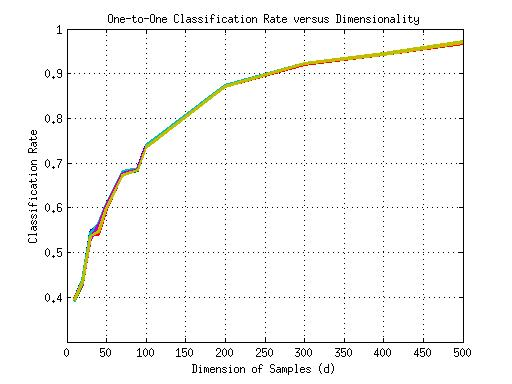
\includegraphics[width=3.3in]{../images/one2one_rate.jpg}
\caption{Classification Rates of the Two Class Classifier using FLDA and One-to-One Strategy. Classification rates for both Euclidean and Mahalanobis distance along with the three ambiguity resolution methods are graphed.}
\label{fig:one2one_rate}
\end{figure}

\begin{figure}[!h]
\centering
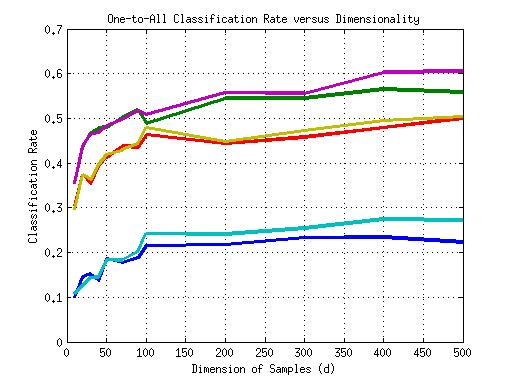
\includegraphics[width=3.3in]{../images/one2all_rate.jpg}
\caption{Classification Rates of the Two Class Classifier using FLDA and One-to-All Strategy. Both Euclidean and Mahalanobis distance metrics are shown here. The blue curves are performance when ignoring ambiguities, the red and orange curves are using the highest prior probabilities to resolve ambiguities and the purple and green curves are using the minimum of the Euclidean distance.}
\label{fig:one2one_rate}
\end{figure}

\begin{figure}[!h]
\centering
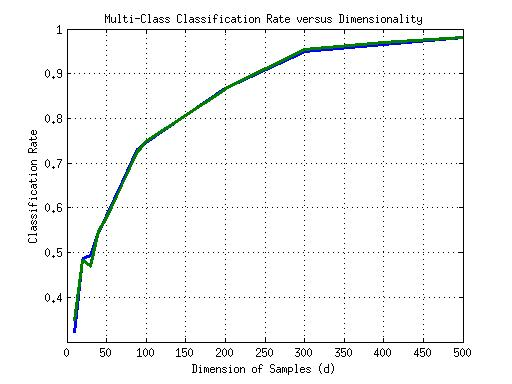
\includegraphics[width=3.3in]{../images/multi_gen_rate.jpg}
\caption{Classification Rates of the Multi-Class FLDA Classifier computed using the Generalized Method. Both Euclidean and Mahalanobis distance metrics are show here. There are no ambiguities using this method.}
\label{fig:multi_gen_rate}
\end{figure}

\begin{figure}[!h]
\centering
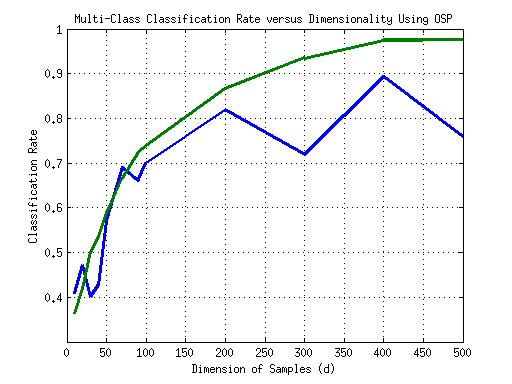
\includegraphics[width=3.3in]{../images/multi_osp_rate.jpg}
\caption{Classification Rates of the Multi-Class FLDA Classifier computed using the OSP Method. Both Euclidean and Mahalanobis distance metrics are show here. The Euclidean distance is the blue curve and Mahalanobis distance is the green curve. There are no ambiguities using this method.}
\label{fig:multi_gen_rate}
\end{figure}

\begin{figure}[!h]
\centering
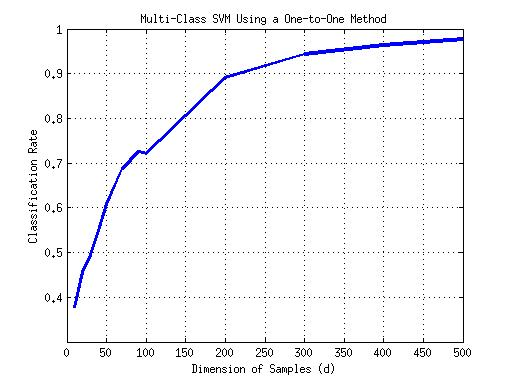
\includegraphics[width=3.3in]{../images/one2one_rate_svm.jpg}
\caption{Classification Rates of the Multi-Class SVM Classifier Using a One-to-one Method. The SVM computes a discriminant function directly therefore there is only one curve.}
\label{fig:multi_svm_rate}
\end{figure}

\begin{figure}[!h]
\centering
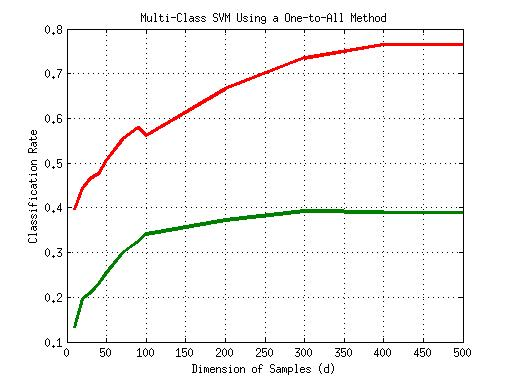
\includegraphics[width=3.3in]{../images/one2all_rate_svm.jpg}
\caption{Classification Rates of the Multi-Class SVM Classifier Using a One-to-All Method. The green curve simply ignored ambiguous classifications while the red curve resolved ambiguities by choosing the class with the closest Euclidean distance to the means.}
\label{fig:multi_svm_rate}
\end{figure}

\section{Algorithm Performance}
\par The performance of each algorithm was assessed by computing the classification rate and number of ambiguous classifications for each classifier over a range of dimensions \(d\). Each test consisted of a minimum number of training samples to satisfy the FLDA model, such that \(N_1=d\), and 1500 test samples. Each training sample provides one constraint when computing FLDA projections. Therefore, it is necessary to have the number of samples in each class be at least equal to or greater than the number of dimensions of each vector. As a result, as we increased \(d\) during testing, we also increased the number of training samples in each class so that class one had at least \(d\) samples.
\par The performance results are given in figures one through six. When studying these figures, it appears that four of the algorithms performed equally well and above the other two. The classifiers designed using the FLDA with one-to-one, the generalized FLDA, the FLDA using OSP and the SVM using one-to-one all performed equally well. The other two classifiers designed using FLDA and one-to-all and SVM and one-to-all performed less well. However, even as the performances of four of these algorithms was more or less the same, there are advantages to some of the classifier designs in terms of computational complexity and number of ambiguous classifications.
\par Among the four that performed well, the FLDA using one-to-one suffered from the largest number ambiguous classifications. As \(d\) increased, the number of ambiguities decreased exponentially. In addition, this strategy for classifier design had the highest computational complexity and running time of all six designs. This is not unexpected as there are \(K \choose 2\) two class problems which must be solved. The SVM classifier employing the one-to-one strategy also has a similarly high computational time, but the number of ambiguous classifications was on the order of zero or one.
\par The multi-class FLDA computed using the generalized method and OSP methods performed equally well when using the Mahalanobis distance metric. When using the Euclidean distance and the OSP method, we encountered a higher variance in the classification rate. When using the OSP method on this particular problem, we encountered some linearly degenerate OSP projections which skewed the FLDA projections. The variability was encountered when using only the first moment of the data to perform classification. When the Mahalanobis distance was used, the classifier performed well. Overall, the Mahalanobis distance metric used to perform classification using FLDA was equal or superior in performance to the Euclidean distance. This is because it takes into account the means and covariances of the projected data which describes the data well. Also, an advantage of these multi-class FLDA classifier designs is that they do not suffer from ambiguous classifications.
\par The two algorithms that performed less well overall were the classifiers designed using FLDA and one-to-all and the SVM using one-to-all. From examining all five projections of the data in the one-to-all classifier, it was obvious that the data was skewed in that for any particular test, the "not class \(C_k\)" had many more samples. Also, the projections of classes \(C_2, C_3, C_4\) overlapped the projections of the other classes. Therefore, the classes became totally unseparable when trying to separate the data. Another observation from the one-to-all strategy is that the Mahalanobis distance metric worked better than the Euclidean distance. This is expected given the large skew in the number of training samples in each category. The variance of the "not class \(C_k\)" was typically much larger than the variance of the "class \(C_k\)" label in the projected space.
\par We employed three methods to help resolve ambiguous classifications. These were used when the one-to-one or one-to-all classifiers resulted in other than one class label assigned to the test sample. The first was to simply ignore the sample and leave it unlabeled. This performed the worst overall because for the one-to-all classifiers we encountered a large number of ambiguities during testing. For example, as high as \(500\) out of \(1500\) tests gave ambiguous results in testing. The second method was to choose the class label which had the highest prior probability. This technique performed better than ignoring the sample as shown in figure 2. Finally, the ambiguity resolving method of choosing the class with the minimum Euclidean distance to the mean performed best overall and considerably improved the results of the one-to-all based classifiers using FLDA and SVM as shown in figures 2 and 6.

\section{Conclusion}
\par In this study we have designed and implemented six classifiers four of which consisted of computing FLDA projections in different ways and using LSE and MLE based distance metrics in the projected space. We extended the two class FLDA projection to design multi-class classifiers using one-to-one and one-to-all strategies as well as the generalized FLDA and FLDA computed using OSP. We also extended LIBSVM to multiple classes using one-to-one and one-to-all strategies \cite{libsvm}. We implemented three ad-hoc ambiguity resolution methods. Of the six classifiers, classifiers based on the the generalized FLDA and FLDA using OSP performed the best, had no ambiguities and were most computationally efficient. While the classifiers based on the one-to-one strategy performed equally well, had few ambiguities but were considerably more computationally expensive. Finally, the two classifiers based on the one-to-all design performed the worst, had a high number of ambiguities, but were more computationally efficient than the one-to-one classifiers.

% References section
\bibliographystyle{plain}
\bibliography{./references}

% Biography
\begin{IEEEbiographynophoto}{Bernard Lampe}
(M'09) became an IEEE Member (M) in 2009 and received his bachelors of science degree from The University of Michigan in Ann Arbor, Michigan, USA in 2009.
\par Mr. Lampe is also a member of the American Society for Computing Machines (ACM) since 2009.
\end{IEEEbiographynophoto}

% End document
\end{document}

